\chapter{Introduction}

Blockchains have enabled a new global market for digital art, allowing artists to publish and sell their work directly to collectors from all over the world, bypassing traditional gatekeepers such as art galleries, auction houses and art dealers. Through chains of cryptographic proofs and consensus protocols which enable public append-only ledgers, blockchains are able to maintain the full history of an artwork's market transactions, from its inception (or \gls{minting}), to its first sale on the \gls{primary market}, and onwards through subsequent transactions on the \gls{secondary market}, and thus natively solve, at least partially, the issue of art provenance, a long-standing problem in the traditional art world. In addition to that, with the use of smart contracts that automatically enforce artist royalties, artists can benefit from a life-long revenue stream, both from \gls{primary sales} and \gls{secondary sales} alike.

As is usual in the art world, when a new technology presents itself, some artists explore its possibilities as an art medium, and blockchain technology was no exception. Artists such as Kevin Abosch, Rhea Myers, Sarah Meyohas, and Sarah Friend, among others, pioneered \gls{conceptual art} using blockchain as a medium, exploring new kinds of interaction between artist, artwork, and collector \cite{rcsBlockchainMedium2022}.

Computational artworks with networking capabilities were made to interact with their environment, and thus evolve over time. However this network capability also brought with it problems. Many code-based artworks become immutable from the moment they are registered on a blockchain, yet the external environment with which they interact keeps changing, and often times those changes are unforgiving for a code-based artefact which cannot mutate to accommodate them, in what can be called a \emph{mutable dependency dilemma}.

This work explores that dilemma, and examines the conservation of networked-based computational art through a technical and cultural lens of \gls{web3}, which is native to the blockchain and crypto community.

This thesis contains many terms which were born out of the crypto community and may be unfamiliar to the reader. Even the term \emph{crypto} itself, with its Greek origins, has been adopted by the cryptocurrency community, thus appropriating a term which until recently had been used mostly by the cryptography community. For this reason this document contains an extensive glossary, starting from page \pageref{sec:glossary}, where many of the terms are defined.

\section{Motivation}

This is not a typical thesis in Information Systems (IS).

The topic presented on this thesis is in fact not the same that I had planned to pursue at the start of the PhD programme.  In the beginning I proposed to build on my Master's degree work, and further develop Grokya, a project which aims to build a personal digital cortex, or an an external digital mind extension \needcite . Such a topic would be purely within the traditional scope of an IS thesis. However after spending half of my allotted research time on such endeavour, I had a change of heart. At that time, the PhD in IS at USJ existed under the umbrella of the Faculty of Arts and Humanities, which was undoubtedly an usual combination. Most IS programmes in other higher education institutions around the world fall under either a Business School, a Faculty of Informatics, or some other Engineering school. I took this unusual mix as an opportunity to pursue a different path for my research. In my personal time I was undergoing a truly transformative experience. As long term member of the cryptocurrency community, I was experiencing first-hand the cultural interchange that was happening between the world of crypto and the world of art. The year of 2021 saw large amounts of artists entering the crypto space as they looked to explore the exciting, and booming, area of cryptoart. At this time I was invited to write a paper for the International Journal of Creative Interfaces and Computer Graphics (IJCICG) and I saw it as perfect opportunity to change my PhD topic, and pursue a theme that truly brought together the world of IS and art. Also for this reason, I spent a good amount of time thinking deeply about what it meant to do research in this interdisciplinary field. I felt as if this thesis, due its unusual placement within the structure of the University, had to do a good job of bridging the Humanities and the Sciences. Ironically, due to a recent restructuring, the University has now moved the PhD in IS programme under the newly created Institute for Data Engineering and Science (IDEAS), which certainly is a more common placement for such a programme. However there was no turning back for me. The research work and the respective thesis presented here represents my attempt at bridging ``the two cultures'' of Science and the Humanities \cite{snowTwoCultures2012a}

To better understand my motivation for this work, as well as contextualise some of the research and development decisions made during the study, it is helpful for the reader to review a brief timeline of my personal experience in the crypto space and how it led to this research topic.

\subsection{Bitcoin}

I first came across Bitcoin in 2011, and experienced the basic use case of installing the Bitcoin-QT software on my laptop and receiving a small transaction (0.02 BTC) from a public faucet ran by early bitcoin developer Gavin Andersen \cite{lucasHowGavinAndresen2022}. As many people at that time, I failed to understand the significance of such a transaction. From a user experience perspective it was underwhelming.  The interface was rudimentary, and the transaction took a while to appear as confirmed. Paypal was miles ahead, or so I thought. This mis-judgement of the merits of the technology due to a very limited understanding, or even complete ignorance, of such a technology is unfortunately very common in the crytocurrency space.

It wasn't until 2013 that I looked into Bitcoin again. This time I read the Bitcoin whitepaper \cite{nakamotoBitcoinPeertopeerElectronic2008} and my world view changed. Technologically the proposition was simple: here is a piece of software which, if enough people run it on their own devices, and adopt it as a legitimate way to communicate value with others, has the potential to redefine the relationship between money, the state, and the people.

As an anarchist sympathetic with the anti-capitalist movement, I brushed aside the fact that Bitcoin was firmly rooted in a capitalist culture, because it also represented a very tangible step away from a financial system which I saw as irreparably corrupt. I became an advocate, organising Bitcoin meetups in Macau \cite{BitcoinMacau2024}, delivering public courses \cite{mouraUSJHoldCourse2021}, appearing in interviews to the media \cite{tdmportuguesenewsprogramsReportagemJornalistaLina2015} \cite{reisBitcoinDuasFaces2017} and generally being very active in the Bitcoin community.

\subsection{Ethereum}

In January 2014, when Ethereum was announced as a concept by Buterin \citeyear{buterinEthereumNextGenerationCryptocurrency2014}, I was instantly impressed. Bitcoin always had basic scripting capabilities baked into its transaction processing logic \cite{ScriptBitcoinWiki2024}, but to take what was mostly a transactional ledger technology and enhance it with a Turing-complete runtime was going to open a world of possibilities. But perhaps even more importantly, Ethereum was also marketed as a decentralised platform where \emph{\gls{code is law}}, a concept which deeply resonated with me. The idea of encoding governance into public, immutable, and self-enforceable rules seemed like a silver-bullet against corruption.

In 2016, a bug was exploited in a smart contract of a DAO which held around 14\% of all ETH in circulation \cite{morrisCoinDeskTurns102023}. Under the \emph{code is law} philosophy, the exploiter only followed the rules of the code, and was therefore the rightful owner of the drained funds. However the Ethereum core developers dismissed the \emph{code is law} mantra and proposed a hard-fork of the blockchain \cite{buterinCRITICALUPDATERe2016} to effectively reverse the attack, salvaging the funds from the hands of the hacker and returning it to their original owners. This was an extremely controversial decision, especially for a space where trustlessness, censorship-resistance, and immutability of transactions are core elements. To make matters worse, in addition to such a significant u-turn in philosophy, the way in which matters were dealt with, much of which documented by an anonymous member of the community \cite{yourstruly1DAOHistoryIt2018}, was very disappointing. Even if Ethereum Classic carried on with the original chain and philosophy \cite{CodeLaw2022}, I was too disillusioned with the crypto space and took a step back.

I should note that more recently I changed my stance regarding \emph{code is law}, as will be explained later.


\subsection{Tezos}

In the summer of 2017 I came across Tezos, a project still in its inception stage, but which was planning to build a self-amending blockchain with a well designed governance system built into protocol, giving its token holders voting power on updates to the protocol itself \cite{goodmanTezosSelfamendingCryptoledger2014a} . 


This was exciting to me because it promised to address the main problem that had led me to exit the Ethereum ecosystem. In addition to that, it would also use a proof-of-stake consensus algorithm from day one, resulting in a much more energy efficient and ecologically friendly blockchain.


Ironically, after delays due to extensive \gls{off-chain} governance issues and disputes between the project co-founders and the president of the Tezos Foundation, who eventually stepped down \cite{irreraExclusiveTezosFounders2017}, Tezos finally launched in September 2018 \cite{daleBillionTezosBlockchain2018}. The delay in the launch is sometimes referred to as a reason why Tezos fell behind other projects in the crypto space, both in terms of developer mindshare as well as overall relevance, in what is a very competitive market.

The following three years saw a modest amount of development around Tezos especially in the areas of \gls{decentralisedfinance} and gaming, however adoption of the chain remained relatively low, as measured by the low transaction volume recorded on-chain, allowing detractors to classify it as a \emph{\gls{ghost-chain}}. In March 2021 all that was about to change.


\subsection{Hic Et Nunc (HEN)}


Hic et Nunc (\indexacronym{hen}) was an NFT marketplace created by Brazilian developer Rafael Silva and launched on the Tezos blockchain in March 2021, becoming the first to do so on that chain, and in the process beating rival marketplace Kalamint, who was still in closed beta.

At a time when the NFT market was experiencing a boom cycle \needcite , many artists, especially those from the Global South, were priced out of the fast increasing gas prices on Ethereum, on account of the high demand for block space. At the same time environmentally conscious artists raised concerns about Ethereum's high carbon footprint, since at that time it still operated on a \gls{proofofwork} consensus algorithm \cite{lemercierProblemEthereumCryptoArt2021}. With Tezos offering very low transactions costs, and also being environmentally friendly due to its \gls{proofofstake} consensus algorithm, HEN's launch on Tezos provided a solution for these two groups of artists, and many others. With an iconic minimalistic and raw interface, the platform invoked an underground culture of experimental and avant-garde digital art. It also intentionally lacked any kind of artist signup process or similar kinds of gatekeeping. Anyone with as little as 0.5 XTZ (approximately \$2.5 USD at the time) in a Tezos wallet could mint an artwork on HEN. After only a few weeks, HEN rose in popularity and by May 2021 it even overtook OpenSea, the largest NFT marketplace in Ethereum, in number of active users \cite{nelsonWhereAreYour2022}. This sudden rise in usage can be clearly seen on the number of transactions and smart contract calls on the Tezos blockchain which started climbing just after March 2021, see \autoref{fig:tezos-tx-vol}. 


\begin{figure}[h]
    \centering
    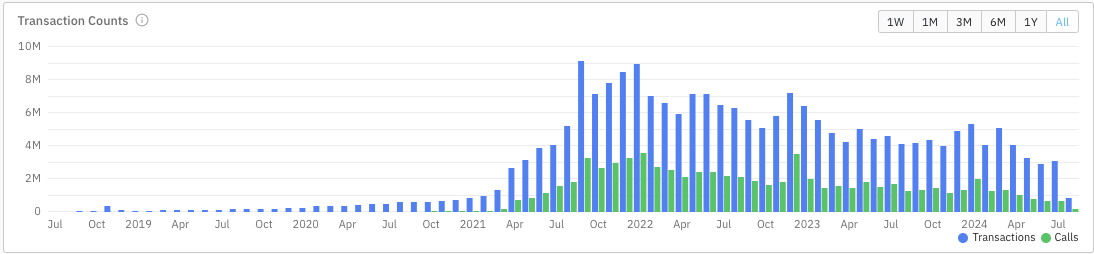
\includegraphics[width=\linewidth]{chart-tezos-tx-volume.png}
    \caption[Transactions per month on Tezos blockchain]{Transactions per month on Tezos blockchain (Jul 2018 - Jul 2024). Source: https://tzstats.com/}
    \label{fig:tezos-tx-vol}
\end{figure}



\subsection{Networked OBJKTs and ``Self-Aware'' Artworks}

HEN named its NFT tokens OBJKTs, so each NFT minted on the HEN smart contract is an \gls{OBJKT} with a unique serial number. The platform supported the minting of OBJKTs using a variety of file formats, and one of those format was SVG (mimetype \texttt{image/svg+xml}). Since the SVG file standard allows for the embedding of JavaScript code, which is executed when rendering the file on a web browser, artists were quick to use this and started minting dynamic code-based artworks, such as ``The Magician'' by Lionel Radisson \cite{makio135Magician2021}




\subsection{TODO}




The research presented in this thesis sits at the intersection between information systems and art. Having started its lifecycle within the context of a PhD program in Information Systems under the umbrella of the Faculty of Arts and Humanities, an usual mix as far as this type of programme is concerned, this research project can best be categorised within the Digital Humanities. 

At the beginning of this journey, the Degree of PhD in Information Systems at the University of Saint Joseph was unusual, in the sense that it was the only PhD programme in Information Systems that I could find which was offered under the umbrella of a Faculty of Arts and Humanities. Every other instance of an Information Systems degree advertised on the Web was either a Management Information Systems (MIS) degree as part of a Business School or a similarly named degree within a Computer Science Faculty. This peculiarity may have been mostly aesthetic, with much of the taught curriculum being in common across all other PhD programmes offered by the University, but I took this uniqueness to heart, and spent a significant amount of time thinking about what it means to research and develop an Information Systems within the context of the Arts and Humanities.

More specifically it focuses on information systems which are ideated, designed and implemented to aid with the discovery and preservation of a fairly new type of digital art: networked cryptoart. 



If art typically already follows, adapts to and reflects technological advances, the opposite cannot be said to happen. One goal of this project is to avoid approaching the issue of \emph{infrastructure} versus \emph{art} as separate things, but rather as a symbiotic relationship where the art and the infrastructure on which it relies complement and inform each other. This means a significant effort was made to study the evolution of digital art in general, with a special focus on netart. 

Prior to blockchain, the print medium was the most reliable way to archive and record one's work, and to build a reference-able portfolio. (Violet Bond in ``The Artist Toolbox'' feat @inWarhol and why being in print matters - https://twitter.com/i/spaces/1OwxWwAPnPkxQ?s=20 )

It is somewhat ironic, that hand prints and other rudimentary paintings on the walls of caves by our pre-historic ancestors are inherently more resilient to degradation than state-of-the-art digital art. We could argue that complexity is the enemy of conservation.


\section{Crypto Culture}


\subsection{Terminology and Definitions}

In this section some of the key terms used throughout this dissertation will be strictly defined.

Web 3 - not to be confused with Web 3.0, a term which has been widely used in a different context, Web 3 refers to a decentralised trust model applied to the web. Although such decentralisation also manifests itself in the architecture of the Web 3 infrastructure, such technical aspect is not by itself its main differentiator from Web 2. After all, Web 2 is also built on a largely distributed computing architecture, with the major technology companies employing large numbers of geographically dispersed datacenter farms, for resilience and speed of access to the users. Web 3 is more concerned with the logical decentralisation of control and political power, rather than the physical decentralisation of computing power.

Crypto attempts to replace hierarchical systems of power, where rules are ultimately enforced by the use of violence, which a non-hierarchical system where ``good'' and ``bad'' behaviours are encouraged or discouraged via economic incentives and/or penalties.

\subsection{Social Contracts, Immutability and Hard Forks}


\todo : explain why I changed my stance on code is law.

This section will focus on one of crypto's core \emph{raisons d'être}, trustlessness.

The term trustlessness, does not mean untrustworthy. Rather it represent's an effort to make trust obsolete, replacing it with transparency and a-priory agreed social contracts. These social contracts, represented by code, both at the blockchain protocol level, as well as written into smart contracts, become immutable agreements, and self-executing rules of engagement. This concept is so deeply engrained into the crypto culture that any scenarios that rely on individual's trustworthiness are only considered when absolutely unavoidable.

Smart contracts play an important role in this concept, because once instantiated in a blockchain they become, by default, immutable. Participants that rely on the smart contract still need to verify that the code does what it is supposed to, and unintended and hard-to-find bugs are not only possible but unfortunately a common occurrence in this early stage of the smart contract industry. Even though these bugs can be exploited, leading to consequences which run counter to the intended social contract, the crypto community accepts this risk and tries to mitigate it with stricter contract development processes, and reviews and verifications. However, a smart contract which is purposefully designed to be mutable (a possibility under some circumstances) or which gives its creator or administrator powers that would require trust by the community on them, are naturally seen with suspicion and even counter to the accepted crypto culture values. In the early days of \indexglossary{ethereum} a name was given to this type of code-based social contract: rule of code.

An important feature of immutable social contracts is that they prevent, or at least minimise, the unilateral ``cheating'' by any participant in a transaction or a serie of transactions. In crypto, the act of cheating other participants is called a ``rug pull'', which means the symbolic act of ``pulling the rug out from under the feet of the victims'' leaving them off-balance and causing them to fall.

Immutability, however, does bring some inconveniences. Some times the immutable code fails to represent the expectation of the social contract, and this can happen for a number of reasons. For example, the code could have an unforeseen consequence due to a bug. Other times the needs of the community change with time and the social consensus evolves in ways which are incompatible with the original code. In some cases this evolution can even cause major fissures in the community, leading to a breakup in consensus, with major splits in the opinion of the best way forward. In these cases the immutable code is unable to adapt to a new reality, and the community has no option but to leave behind the original protocol, and jump to a new, modified protocol. We call this phenomenon a \emph{hard-fork}.

There were notable hard-forks in the history of crypto (mention BTC/BCH, ETH/ETC, etc)

Perhaps most importantly is that every participant in an activity is satisfied that their expectations are met by the system, and where opinions between them evolve and diverge, that the system provides a satisfactory and fair resolution to all stakeholders. 

\subsection{Why Decentralisation?}
(looking for a better heading. why do we need trustllessness, immutabilty, censorship resistence, etc)

Activism through digital art, see \cite[p.~212]{hopeDigitalArtsIntroduction2014} , benefits greatly from low barriers of entry, lack of gatekeepers, and censorship resistance (both as infra resilience, and social structures), but how can it be counter-balanced with curation of content, policing of copy mints or copyright infringement, removal of illegal material (i.e. child porn, etc).

Decentralisation as a way to remove single-points-of-failure, thus resilience to attack, was an intentional design decision of ARPANET, which led to the Internet we know today. \cite[p.10]{paulDigitalArt2015}


\section{Definitions}

crypto-art
computer art
algorithmic art
generative art
code-based art
time-media art
netart
telematic art
interactive art
digital art
software art
new media art


electronic art
computational art
new media art
multimedia art
internet art
digital installation art
immersive art,
CGI (computer-generated graphics)
digital illustration
graphic design


\section{A New Type of Art}

This thesis invites readers to look at networked art under a new light of sensorship-resistant long-lived preservation, powered by decentralised technologies. Rather than create its own visual aesthetic, this new kind of art may be characterised by a common set of processes and underlying architectures that afford it with the kind of long-lasting characteristic that is seldom attributed to digital medium art.
Another factor that distinguishes it from previous net art is the ability of art pieces to be ``aware'' of their own existence in the marketplace, allowing them to react to actions such as being put up for sale, being sold, the monetary amounts involved, who owns them, etc.
In theory, a piece of art could be created in such a way as to 'earn' a stipend from each sale, and through its own trading activity eventually earn enough as to be able to 'purchase' itself from its human owners, and gain some sort of freedom, or emancipation.
Futhermore, it attempts to blend the seemingly conflicting forces of preservation and evolution.

\subsection{Art as Revolution}

``If revolution can give art its soul, then art can give revolution its mouthpiece'' - Anatoly Lunacharsky

TODO: Refer to ``Art and Revolutio'' by Gerald Raunig (available in UMAC lib: NX 180 R45 Rau 2007)

Walter Benjamin hailed the liberatory and transformative effects of mechanical reproduction on art, suggesting that ``mechanical reproduction erodes the 'aura' of a work of art, which results from its unique existence in a time and place, which revolutionized the social function of art and allowed it to be used for politics rather than ritual''. (Benjamin, 2002: 103-6 - cited in \cite[p.3]{gereArtTimeTechnology2006}

\section{Contributions}

This thesis contributes to the body of knowledge in the following ways:

It proposes a new taxonomy for categorizing xxx which takes into account yyy, and zzz.

Using this new taxonomy an extensive review and categorization of xxx was undertaken and is available online at https://abc.xyz

It contributes to the field of digital art preservation by combining xxx with yyy in a novel way, and provides evidence of its efficacy in findings nnn.

It demonstrates de economic viability of running decentralised infrastructure by incentivising xxx via the use of zzz, as seen in chapter yyy.

In the field of information systems, it studies and reports on the application of xxx and yyy in the context of zzzz

In conducting the research, the efficacy of using methodology xxx was tested in the context of uuu, revealing limitations yyy and zzz.

Last but not least, it proposed a new paradigm for art creation based on xxx, and extensively tested its limitations. In doing so, it also raised important questions that should inform future research efforts. Namely, xxxx.

Digital assets like \gls{nonfungibletoken} are transforming the art world. An \indexacronym{nft} is a unique digital asset verified using blockchain technology.
This document discusses various examples (EX) of digital assets and their conservation techniques. This is the nature of the \gls{nonfungibletoken}.


\section{Conservation}

Mention how the Internet Archive, in cooperation with the MAME project, which started as an emulator for old arcade games, has now branched to include other kinds of vintage hardware, like consoles and even scientific calculators. \cite{scottjasonCalculatedMoveCalculators2023}

This is a quick mention of \gls{emulation} so that it appears on the glossary.


\subsection{Historical Consensus - Conservation of Bugs}

One interesting side-effect of maintain global consensus is that every full node must independently validate the whole chain, from it's genesis block until the latest block, which is commonly called the ``head'' of the blockchain. This means every full node, no matter how recently implemented, must be able to replicate every historical consensus rule, including any bugs in early node software, such that all historical block validation proceeds exactly as it did originally. Failure to replicate such bugs would potentially result in modern nodes considering historical blocks as invalid, hence refusing to follow the main historical chain and therefore forking the chain.

\subsection{Value of information}

Information has economic value because it allows individuals to make choices that yield higher expected payoffs or expected utility than they would obtain from choices made in the absence of information (must rephrase this, was taken from wikipedia).
We live in an era of asymmetric access to data, with those with access in adversarial position to the individuals to which the information pertains. 


\section{Blockchain Interactivity}



\subsection{Burn it: NFTs as reedemable vouchers}

One of the most common interactions between collectors and projects is the act of collecting and burning tokens as a way to unlock other features in the project, access special drops, or others. Collectors have to weigh in the cost-opportunity of destroying a token in exchange for another which may, or may not, be more desirable for them, both from an economic and aesthetical point of view. Whilst creating an environment of engagement and gamification of the project, it can certainly be considered one of the most striking examples of commodification or art in the NFT world. The very act of permanently disposing of a piece of art in return for some kind of utility is arguably against the very ethos of ``art'' (that which has no utility).

The topic of utility has itself generated a fair amount of debate among the cryptoart enthusiasts. TODO: expand on this.

\subsection{Bootloader method}

A web3 approach is to load a lightweight bootloader OBJKT, which is able to contact the blockchain for the IPFS hash of the latest version of the artwork.

\begin{figure}[H]
  \centering
    \scalebox{1}
    {  \begin{sequencediagram}
    \newinst{browser}{\shortstack{User \\ Browser }}{}
    \newinst{marketUI}{\shortstack{Marketplace \\ UI }}{}
    \newinst{indexer}{\shortstack{Blockchain \\  Indexer }}{}    
    \newinst{ipfs}{\shortstack{IPFS \\  Gateway}}{} 
    \begin{call}{browser}{ }{marketUI}{1. page UI}
    \end{call}
    \begin{call}{browser}{ }{indexer}{2. OBJKT metadata}
    \end{call}
    \begin{call}{browser}{ }{ipfs}{3. OBJKT payload}
    \end{call}
    
  \end{sequencediagram}
  }
\caption{Loading a non-networked OBJKT - HTTP request sequence} 
\end{figure}

A networked OBJKT also starts with the same 3-step loading sequence as its non-networked variant, but it makes additional requests to load data from external data sources. See figure \ref{fig:objkt-loading-net}.

\input{figures/objkt-loading-net}

It is these additional network calls by the loaded OBJKT that can easily stop working, because unlike steps 1-3, which are controlled by the page UI and are therefore editable by the marketplace, the OBJKT payload is immutable from the moment of minting, and hence cannot accommodate any changes to any elements of these last requests, may they be in the URL, API changes, or any others.

We should also mention \indexacronym{nft}s here to see if the glossary updates itself.


